\chapter{Long-distance communication}
\label{sec:11_long-distance}

In this chapter, we will give you the context of how we can communicate over long distances in classical networks, and see how that fits within the context of quantum communication as well.

\section{Introduction}
\label{sec:ld-intro}

% Hi, and welcome to Lesson Eleven on Long Distance Communication.

Let's go back to the year 1852 and consider a little bit of the historical background of long-distance communication.

\begin{table}
\centering
\begin{tabular}{|c|c|}
\hline \multicolumn{2}{|c|}{ Letter from London ${ }^*$} \\
\hline to & took [days] \\
\hline New York & 12 \\
Bombay & 33 \\
Singapore & 45 \\
Sydney & 73 \\
\hline
\end{tabular}
\caption{Prior to the invention and deployment of the telegraph, long-distance communication was slow.}
\label{tab:london-letter}
\end{table}

Just before the widespread deployment of the telegraph, communication was extremely slow. To give you some idea of how slow it was, if you wanted to send a letter from London, let's say to New York, it took around twelve days to arrive, as shown in Tab.~\ref{tab:london-letter}. If you wanted to send it to Sydney, then you had to wait seventy three days for the letter to be delivered. The first long-distance telegraph line, made of copper wire, stretched over land from Washington to Baltimore, but the telegraph immediately sparked the dream of a transatlantic submarine cable. People realized that if they can use the telegraph to communicate over land so quickly, they should be able to connect continents with submarine cables as well. So in 1850 the very first submarine telegraphic cable was laid, connecting England and France. That worked fine, so immediately people wanted to lay a cable across the Atlantic Ocean. For the next fifteen years there were many failed attempts, but this sparked a focused mathematical analysis of very long distance communication. \rdv{tell me more...?}. Although one cable functioned long enough for Queen Victoria of the United Kingdom and President Buchanan of the United States to exchange messages in 1858, it wasn't until 1866 that the first truly successful transatlantic telegraphic cable was laid and used~\footnote{This preceded the first transatlantic radio communication by thirty-five years.}. By 1871, only few years later, all of the continents except Antarctica were connected.

Then, between 1902 and 1906, the first transpacific cables were laid, connecting mainland US with Hawaii, Guam, and later Philippines, and finally Japan~\footnote{rdv finds it an interesting historical anecdote that one of Japan's first undersea cables came ashore in the seaside town of Kamakura, where he lives, in 1931.  It connected to Midway, Hawaii, then the continental U.S.  It was in use for around a dozen years.}. After the telegraphic cables came telephone cables, and in 1956 we had the first transatlantic telecommunications cable, called TAT-1. This coaxial telephone cable initially was able to handle 36 concurrent telephone conversations, later upgraded to 72. 
Compare that with the state two decades later, when the last of the coaxial copper 
%\rdv{dedicated? analog? coaxial? non-fiber?} 
telephone cables, TAT-7, was in use. It could handle a staggering 4000 telephone conversations concurrently. After this came the fiber optic cables. As we saw in Ch.~\ref{sec:7_waveguides}, in 1988, the first transatlantic fiber optic cable, called TAT-8, was laid and increased the bandwidth to the equivalent of forty thousand telephone conversations.

All of these cables, both copper coaxial cables as in TAT-1 through TAT-7 and fiber optic cables from TAT-8 to the present day, carry more than one conversation over a single physical connection.  The earliest telephone wires, in the nineteenth century, supported only a single conversation, because they used \emph{baseband communication}\index{baseband communication}. In baseband communication, the signal to be sent is, well, sent on the wire, unadorned.  If you want to send a 3kHz sine wave, then the wire carries your 3kHz sine wave. This requires one physical connection for every concurrent conversation, which obviously incurs enormous cost.  It would not be practical to have one pair of copper wires for each phone conversation crossing the Atlantic.  Instead, \emph{signal modulation}\index{signal modulation} is used.  The original data signal is used to modulate, or modify, a \emph{carrier signal}\index{carrier signal}. For example, if your data signal is just binary data, the simplest form of modulation might be \emph{on-off keying}\index{on-off keying}, where the carrier is simply turned on and off, like blinking a light. For both analog and digital data signals, many modulation schemes have been developed, but this topic is beyond the scope of this book. See the "Further Reading" at the end of the chapter block for more.  Generally speaking, the carrier signal must be a higher frequency than the baseband signal you are modulating. By using separate carrier frequencies, we can have a copper cable or optical fiber carry more than one conversation at the same time. These frequencies are divided into \emph{channels}\index{channel (frequency or wavelength)}~\footnote{In this book, usually when we use the term "channel", we are referring to the physical fiber or connection, instead of this frequency-based concept.  Sometimes, we are referring to an abstraction that carries a qubit through space or time, usually in the context of error analysis and correction, as in "bit flip channel".}.  This is a form of \emph{frequency division multiplexing}, or FDM\index{frequency division multiplexing (FDM)}, the same scheme used for radio stations and television channels. When applied to fiber optics, this technique is usually referred to as \emph{wavelength division multiplexing} (WDM)\index{wavelength division multiplexing (WDM)}, instead of FDM.  We will see other multiplexing schemes for sharing physical resources in the next chapter.

In this chapter, we are going to focus on the main considerations when designing these cables, particularly bandwidth and noise.

Bandwidth tells us basically how much information a cable or fiber can carry.
This depends on both the physical properties of the fiber itself, as well as how clever we are when it comes to encoding this information before it gets transmitted. With modern techniques such as dense wavelength division multiplexing (DWDM), we are able to reach some staggering speeds. For example, in a standard cable over the distance of 6,600 kilometers, we can reach speeds of something like 65 terabits per second. In a more specialized cable and over shorter distances, this can be increased to over 150 terabits per second. Over very short distances, we achieved speeds of one petabit per second. This is something incredible! (A terabit, just for your reference, is $10^{12}$ bits, while a petabit is $10^{15}$ bits.)

Of course, no system is a hundred percent efficient, and what we put in is not exactly what we're going to get out at the end of the cable. We must consider the main sources of loss in optical fibers. We will consider the following five losses: dispersion, absorption, scattering, bending, and coupling. The combined result of all of these sources of loss is that our signal becomes \emph{attenuated}\index{attenuation}, meaning if we put some signal as an input with some power, what we get out as the output will have less power. It's very important to know how much of the signal becomes attenuated and how we can prevent this attenuation or combat this attenuation.

Another important factor that affects how much the optical signal is attenuated is the wavelength of the light used for encoding.
Different wavelengths have different absorption coefficients.
This naturally makes certain wavelengths more suitable for long-distance communication.
The main three wavelengths used for fiber optic communication are near 850, 1300, and 1550 nanometers, which all lie in the infrared spectrum.
The wavelength of light is important in quantum communication for other reasons as well.
Not all sources of light can produce single photons of the desired wavelength, detector efficiencies depend on the wavelength of the photons, and quantum memories can couple to light only in certain wavelength regions. When multiple connections (whether classical or quantum) share the fiber, they are assigned separate wavelengths. If the assigned wavelengths are too far apart, then fewer channels can be carried; if they are too close together, \emph{filtering}, or selecting out, the desired channel is hard and inter-channel interference becomes a problem. 
All these factors introduce extra complications which must be accounted for when designing and implementing quantum networks.

In this chapter, we will first talk about the dispersion in optical fibers, then we will consider the other sources of attenuation. Then we will move on to overcoming these losses, and finally we will consider the challenges these sources of loss present in the context of quantum communication.


\section{Mode dispersion}
\label{sec:11-2_mode_dispersion}

\begin{figure}
    \centering
    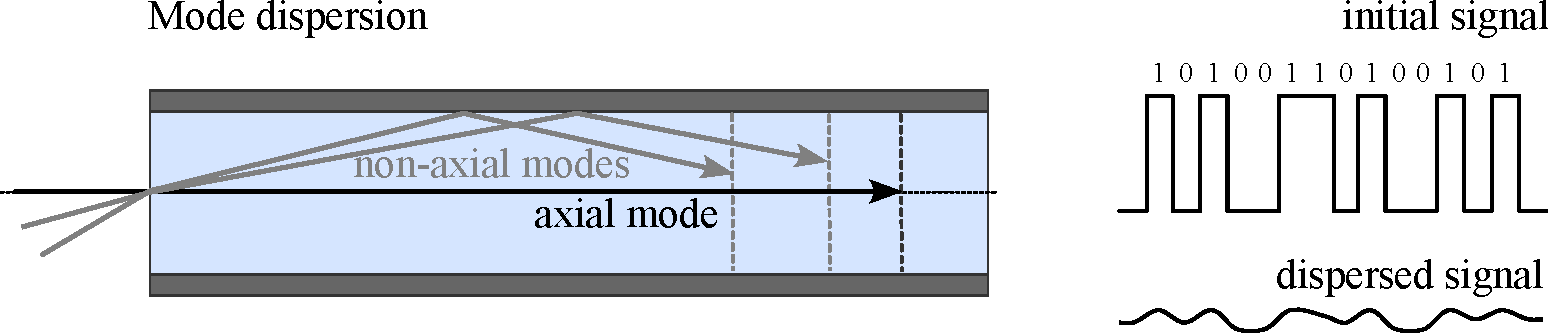
\includegraphics[width=\textwidth]{lesson11/11-2_dispersion.pdf}
    \caption[Mode dispersion]{Different modes traverse the length of the fiber in different times, leading to mode dispersion. Initially sharp signals become difficult to decode.}
    \label{fig:11-2_mode_dispersion}
\end{figure}
Mode dispersion\index{mode dispersion} is the first source of signal degradation in the fiber that we're going to consider.
Let's consider the propagation of different modes in a multimode fiber\index{multimode fiber}, as in Fig.~\ref{fig:11-2_mode_dispersion}.
A multimode fiber can contain many modes, all traveling with different paths. For example, you can have the axial path which travels directly down the fiber, or you can have other modes which totally reflect internally within the fiber. And as you can see, the different modes propagate down the fiber at different speeds because they have to traverse different lengths. It's very important to compute the time difference introduced by the different modes traveling at different speeds down the fiber, and as you might expect, this depends on the launch angle. Depending on the angle with which the light is coupled to the fiber, the path that it takes will be different, and therefore the time that it takes that mode to traverse the fiber will be also different.

The fastest mode, as you can clearly see, travels directly down the center of the fiber. This is known as the \emph{axial mode} because it travels down the axis of the fiber. The slowest mode is the one that is incident on the cladding just at the critical angle, meaning it just barely gets internally reflected.

Your initial digitized signal may look something like the clean modulated square wave in the uppere right of Fig.~\ref{fig:11-2_mode_dispersion}. It's very sharp and it's very easy to read out when you have a zero and when you have a one. But as the different modes propagate down the fiber, the whole packet will spread and disperse. After some distance, it will look something like the bottom right of the figure.
This means that the readability of the output signal worsens, meaning it's more easy to make a mistake when you're actually trying to decode your signal after it propagates through the fiber.

\begin{figure}
    \centering
    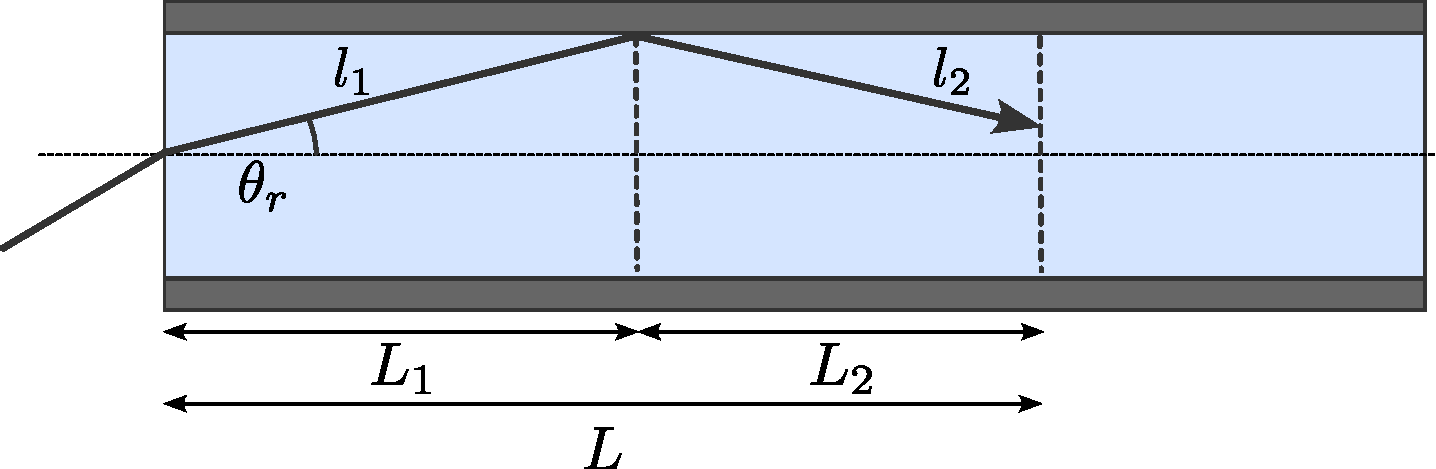
\includegraphics[width=0.8\textwidth]{lesson11/11-2_dispersion_delay.pdf}
    \caption[Time delay due to mode dispersion]{Time delay due to mode dispersion.}
    \label{fig:11-2_dispersion_delay}
\end{figure}

\michal{I started the rewrite from here until the end of this section.}
How quickly this dispersion occurs can be quantified by the time between the fastest mode and the slowest mode.
We're going to consider a horizontal length $L$ that the fastest axial mode traverses. The time that it takes for this mode to traverse this distance is $t_{\text{min}}$,
\begin{equation}
    t_{\min } =\frac{L}{v_f}.
\end{equation}
The speed of of light in the fiber depends on the fiber's refractive index, $v_f = c / n_f$.
Therefore the minimum time can be written as
\begin{equation}
    t_{\min } =\frac{Ln_f}{c}.
\end{equation}

Before considering the time $t_{\max}$ that the slowest mode takes to cover the horizontal distance $L$, we consider a general non-axial mode as shown in Fig.~\ref{fig:11-2_dispersion_delay}.
The total distance $l$ that this mode travels is larger than $L$.
The distance travelled before the internal reflection is $l_1$, and the distance traveled after the internal reflection is $l_2$.
Naturally, we have $l = l_1 + l_2$.

Let's start by computing $l_1$,
\begin{equation}
    l_1=\frac{L_1}{\cos \theta_r},
\end{equation}
where $\theta_r$ is the angle of refraction at the interface between the core of the fiber and the fiber's surroundings.
A similar expression is true for $l_2$, namely $L_2 / \cos \theta_r$.
Therefore, the total distance that the light travels is given in terms of the axial distance $L$ and the angle of refraction $\theta_r$,
\begin{equation}
    l=\frac{L_1}{\cos \theta_r}+\frac{L_2}{\cos \theta_r}=\frac{L}{\cos \theta_r}.
\end{equation}
The time needed for this non-axial mode to cover the horizontal distance $L$ is
\begin{equation}
    t = \frac{l}{v_f} = \frac{L}{v_f \cos \theta_r} = \frac{L n_f}{c \cos \theta_r}.
    \label{eq:11-2_time_nonaxial}
\end{equation}

We are now in position to compute $t_{\max}$.
The slowest mode is the one that has to cover the longest distance $l$.
In order for this to happen, the angle at which this mode is incident at the cladding is maximized while still being completely reflected.
The mode needs to be incident at the cladding at the critical angle $\theta_c$, which in turn fixes the maximum angle of refraction such that
\begin{equation}
    \cos\theta_r = \sin\theta_c = n_c / n_f,
    \label{eq:11-2_cos_theta_r}
\end{equation}
where the last equality comes from Eq.~(\ref{eq:7-4_crit_angle}).
Substituting for $\cos\theta_r$ in Eq.~(\ref{eq:11-2_cos_theta_r}), we obtain the time it takes for the slowest mode to traverse the horizontal distance $L$,
\begin{equation}
    t_{\max }=\frac{L n_f^2}{c n_c}.
\end{equation}
Now it's very easy to just put the expressions for $t_{\mathrm{max}}$ and $t_{\mathrm{min}}$ together, and we obtain the time delay between the fastest and slowest modes, 
\begin{equation}
    \Delta t = t_{\max} - t_{\min} = \frac{L n_f}{c}\left(\frac{n_f}{n_c}-1\right).
    \label{eq:11-2_time_delay}
\end{equation}

Let's consider an example to gain some intuition about time delays introduced by mode dispersion and their effect on the encoded message.
Let's consider a fiber with refractive index $n_f = 1.500$, and cladding with refractive index $n_c = 1.489$.
Using Eq.~(\ref{eq:11-2_time_delay}), we obtain the following time delay per kilometer,
\begin{equation}
    \frac{\Delta t}{L}=37 \mathrm{~ns} / \mathrm{km}.
\end{equation}
This doesn't seem like much.
Let's see the consequences of this small delay.
The speed of light in this fiber is given by $c$ divided by the refractive index of this fiber, which is just $v_f=c / n_f=2 \times 10^8 \mathrm{~m} / \mathrm{s}$.
This time delay between the fastest and slowest modes means that our pulse spreads over a distance as it travels through the fiber. We can quantify this dispersion and obtain the value $7.4$ meters per kilometer -- our slowest signal is about three-quarters of one percent slower than our fastest. Every kilometer that our signal travels, it becomes more and more spread by this distance, $7.4$ meters.
%This reduces the readability of the output signal. 
Because our wave packets are becoming more spread out, we are losing the sharpness of our signal and they become more difficult to decode. In order to be able to read our output signal, we may demand that the pulses that are coming out of our fiber are separated by twice the value of the spread.
This means that in order for the dispersed signal that's coming out of the fiber to be intelligible, we require that the input pulses are also separated by at least $2\times 7.4 = 14.8$ meters even when connecting over a distance of only one kilometer. This inadvertently places a limit on how fast we can transmit information because the pulses have to be separated by a certain amount.
%, so we cannot place them closer together. 
Dispersion has a direct consequence on the maximum frequency of the input signal.



\section{Attenuation}
\label{sec:11-3_attenuation}

\begin{figure}[t]
    \centering
    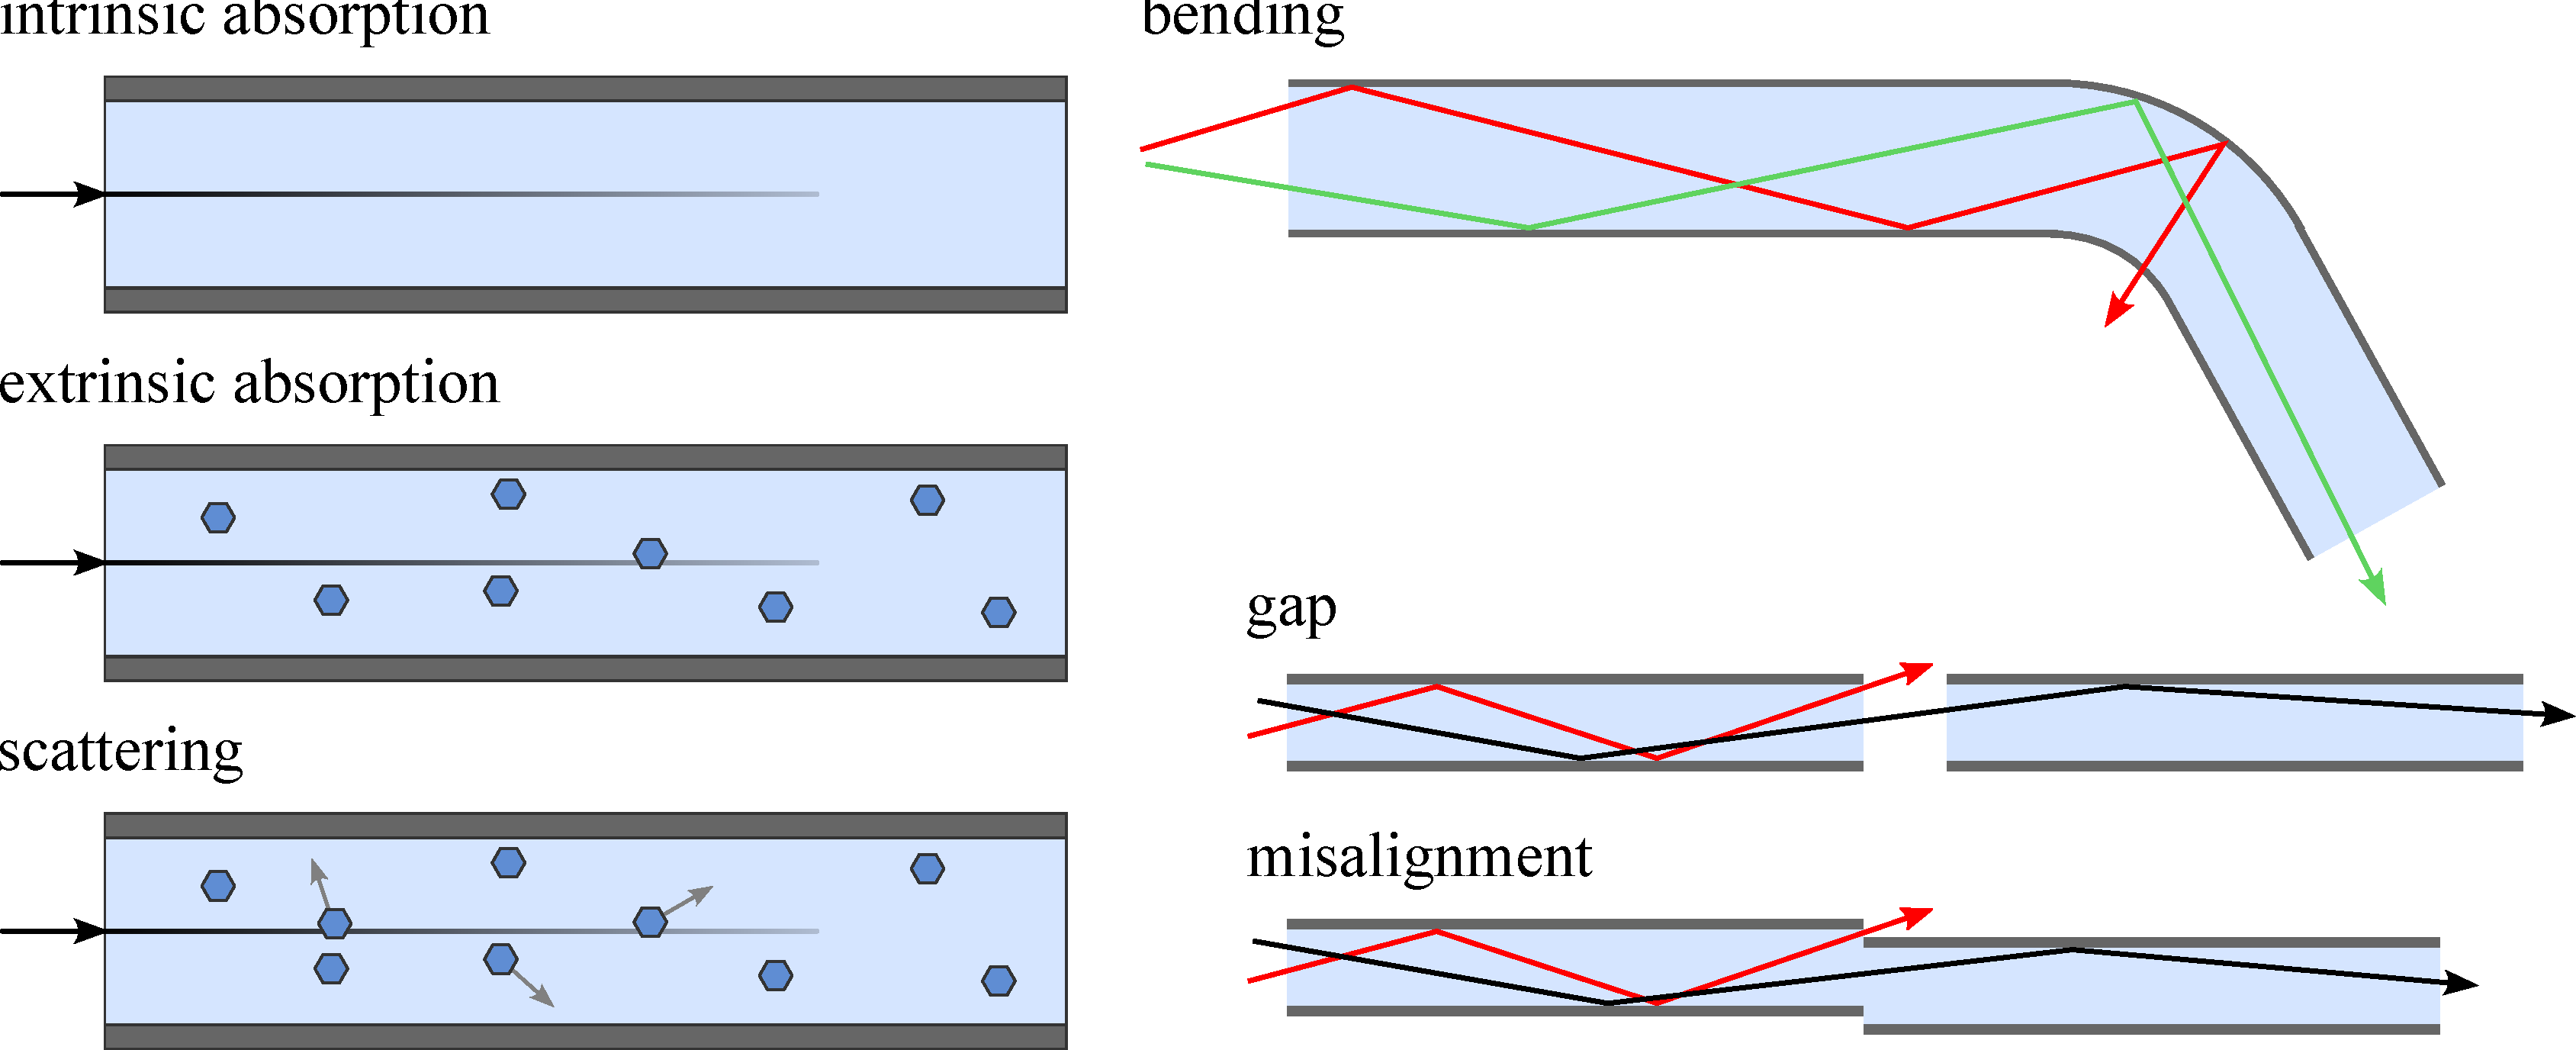
\includegraphics[width=\textwidth]{lesson11/11-3_attenuation.pdf}
    \caption[Attenuation losses]{Various types of attenuation losses.}
    \label{fig:11-3_attenuation}
\end{figure}
In this section, we will consider the rest of the sources of losses that we listed in Sec.~\ref{sec:ld-intro}.
They are all pictured in Fig.~\ref{fig:11-3_attenuation}.

First, let's look at \emph{absorption}\index{absorption}.
Absorption happens due to interaction of light with the material of the fiber. There are two types of absorption: \emph{intrinsic absorption} and \emph{extrinsic absorption}. Intrinsic absorption is responsible for attenuating the signal due to electronic and vibrational resonances of the molecules in the fiber. For silica molecules, electronic resonances occur in the ultraviolet region, and vibrational resonances in the infrared region. These resonances cause the light to transfer it energy to the molecules in the fiber resulting in a power loss in the signal. This is an intrinsic property of the fiber and we cannot really affect it, it's something that we just have to live with and accept. But luckily, it's not a very significant source of error, especially when we compare it to the other type, extrinsic absorption.

Extrinsic absorption is due to impurities in the form of bubbles that are present in the fiber and were introduced during the manufacturing process. On one hand, this is a much more significant source of absorption, but on the other hand we can control it by perfecting our manufacturing process. Generally during manufacture, the manufacturers are trying to keep the the amount of impurities that are present in the fiber below one percent.

Another source of attenuation is \emph{scattering}, which can be due to small fluctuations of the density in the fiber material which are introduced during manufacturing process.
This results in a non-uniform refractive index in the material causing scattering of light.
Other sources of scattering include molecules absorbing the light and re-emitting it in a random direction.

The final two sources of attenuation are \emph{bending} and \emph{coupling}. Bending is when we actually physically bend the fiber. Remember, we said that the angle of incidence is crucial for total internal reflection to take place, and therefore for the signal to propagate down the fiber. If we bend the fiber, we can have a situation where at first, the light ray is traveling down the fiber totally internally reflected but then it hits the angle at the bend and suddenly at the interface it is reflected in such a way that it cannot satisfy the condition for total internal reflection anymore, and it just gets absorbed or it leaves the fiber.  Generally, the manufacturer specifies some minimum bending radius, typically around ten to twenty times the diameter of the fiber.

The other source of error is the coupling error. Inevitably, we will have to join two fibers together, and if there's a gap between the fibers, then the light can of course escape. Another source of coupling error is when the fibers are not aligned properly, so even if there is no gap but they are slightly misaligned as in Fig.~\ref{fig:11-3_attenuation}, then light is allowed to escape and leave the fiber, and the overall signal will become attenuated.

Now that we have discussed the main sources of loss, let's discuss how to quantify the attenuation in a fiber.

As the signal propagates through the fiber, it loses power, so we need to quantify how much power it lost. This is done by a unit called the \emph{decibel}\index{decibel}. The decibel designates the ratio of the two power levels: the power in and the power out.

The number of decibels is defined as the following expression:
\begin{equation}
\# \text { of } \mathrm{dB}=-10 \log _{10} \frac{P_o}{P_i}
\label{eq:decibels}
\end{equation}
where $P_i$ in the power in and $P_o$ is the power out. Remember, the power out has to be less than power in, because the signal is getting attenuated.  Because this ratio is less than one, the logarithm is negative, so applying a minus sign lets us talk in terms of positive numbers. For convenience, we multiply by ten ("deci" means ten) and talk about decibels. Why take the logarithm? Because we will be considering a large span of orders of magnitude between the power in and the power out, and therefore if we take the logarithm, then it will produce a sort of generally nice scale for the number of decibels.  Moreover, since every kilometer of fiber multiplies the power loss, using this logarithmic scale we can easily calculate total loss when we know the distance.

\begin{table}
\centering
\begin{tabular}{r|c}
$P_o: P_i$ & $\mathrm{~dB}$ \\
\hline $1: 10$ & 10 \\
$1: 100$ & 20 \\
$1: 1000$ & 30
\end{tabular}
\caption{Examples of calculating loss in decibels (dB).}
\label{tab:decibels}
\end{table}

For example, if we have the ratio of power out to power in as $1:10$, meaning that ninety percent of the power is lost to attenuation, then this corresponds to ten decibels (10dB), as you can convince yourself by substituting for $p_0/p_i$ into Eq.~\ref{eq:decibels}. If the ratio is $1:100$, then this corresponds to twenty decibels (20dB); if it's $1:1000$, this corresponds to thirty decibels (30dB). You can see that when the ratio of the power out over power in shrinks by an order of magnitude, the loss in decibels increases by adding ten. This calculation is just linear due to the definition in terms of the logarithm.

We can define the attenuation parameter $\alpha$ to be the number of decibels per kilometer, so $\alpha$ is just our previous expression divided by the length of the fiber $L$. We can now rearrange it and get an expression for the fraction of the power out over power in,
\begin{equation}
\begin{aligned}
\alpha & =-\frac{10}{L} \log _{10} \frac{P_o}{P_i} \\
-\frac{\alpha L}{10} & =\log _{10} \frac{P_o}{P_i} \\
\frac{P_o}{P_i} & =10^{-\alpha L / 10}.
\end{aligned}
\end{equation}

We said in the previous chapters that in 1970, optical fiber managed to transmit just $1\%$ of the power that was put in over a distance of one kilometer. We can now just plug that into our formula, and we will find that $\alpha$, the attenuation parameter, is twenty decibels per kilometer (20 dB/km). Two decades later, the transmission rose to around $96\%$ over a kilometer, which corresponds to an attenuation level of 0.18 dB/km. Three decades on, attenuation levels remain around this value.

\begin{figure}
    \centering
    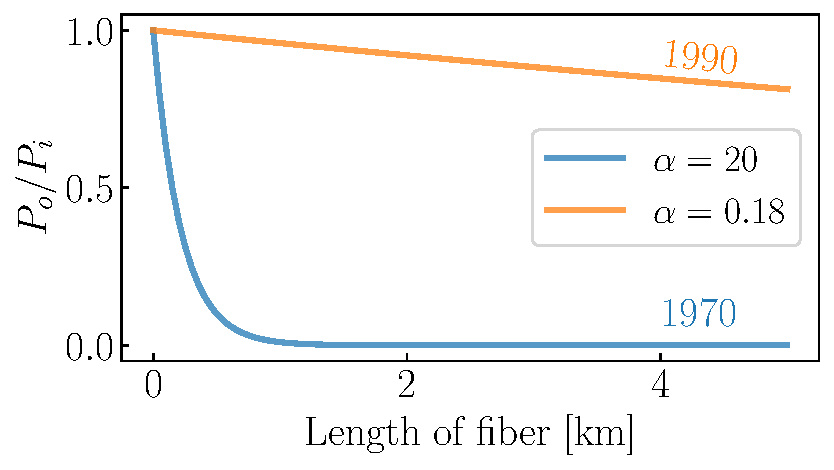
\includegraphics[width=0.6\textwidth]{lesson11/11-3_attenuation_dB.pdf}
    \caption[Power loss in fiber]{Loss in the fiber with distance has improved substantially.}
    \label{fig:11-3_attenuation_dB}
\end{figure}
Figure~\ref{fig:11-3_attenuation_dB} shows the loss versus distance for these two values of attenuation loss. On the horizontal axis, we plot the length of the fiber through which our signal is traveling, and on the vertical axis we have the ratio of the power out over power in. If the length of the fiber is zero, then of course the ratio is one. Our signal hasn't traveled anywhere, so it didn't have chance to be attenuated. As it travels through the fiber, the blue line corresponds to the attenuation levels that were achieved in 1970, with $\alpha$ set to twenty decibels per kilometer, while the orange line is the attenuation levels achieved  in 1990 with $\alpha$ of 0.18dB/km. We can see that how quickly the ratio approaches zero for the high attenuation parameter, whereas for the very low attenuation parameter it decreases much more slowly.

Now that we know what the main sources of loss are and how to quantify them, how can we counteract these losses in our fiber?

\section{Overcoming losses}
\label{sec:11-4_overcoming_losses}

We have seen what the sources of losses are. Now, let's discuss how we can overcome them.

Let's look at dispersion first, that's probably one of the easiest. We saw that the signal and the different modes become dispersed in a multi-mode fiber, but this is not the case in a single-mode fiber, where there is only one mode so there's nothing to be dispersed. Therefore, if in some situation mode dispersion is a big source of error, it's best to switch to a single-mode fiber. We saw that absorption and scattering can be reduced by improving the manufacturing process because the main source is the impurities in the fiber. Bending loss, of course, is reduced by not bending your fiber unless you absolutely have to, and even then being very mindful of how much you bend it. And finally, coupling errors can be eliminated, at least partially, by ensuring that the fibers are aligned properly and there is no gap between them. But even if we try to do all of these things, there will be still some attenuation and some losses, so let's go back to our expression for how much power we lose for some input power over a distance $L$ with some attenuation parameter $\alpha$.

No matter how careful we are about the manufacturing and using single-mode fibers and coupling the fibers together in a proper way, we will always have the attenuation parameter $\alpha$ be non-negative. Therefore, there will be some attenuation on the signal. In the previous section, we saw how much the signal becomes attenuated over a short distance of five kilometers, if the $\alpha$ parameter is set to something very low, like 0.18. The signal becomes attenuated, but not by that much: still around 80\% of the signal gets through, but five kilometers is not a very long distance. Let's try to extend this distance and see what happens. If we extend it to something like a hundred kilometers, immediately you see that even in a low-loss fiber that has $\alpha$ parameter of 0.18, eventually the signal will go to nearly zero. After twenty kilometers, it's around 44\% of the initial power. After only fifty kilometers, it drops to 13\%, and at the distance of a hundred kilometers it is virtually zero. A hundred kilometers is not such a long distance; we need systems that can reach thousands of kilometers. So the question is, how can we use fiber optics to actually transmit signals over such extreme long distances?

Long-distance transmission is achieved with the help of \emph{repeaters}\index{repeater (classical)}~\footnote{Just to remind you, we will encounter this term "repeater" in the next chapter as well, where we will be talking about quantum repeaters, but they work on a very different basis than classical repeaters. Here, we are talking only about classical repeaters.}, which are devices that are used to boost the signal strength. There are many different kinds of repeaters based on many different physical principles. In this chapter, we are going to talk about \emph{erbium-doped fiber amplifiers}\index{amplifier}, or EDFA\index{erbium-doped fiber amplifier (EDFA)} for short. To build one, you introduce erbium atoms into a stretch of fiber. To use it, you pump the erbium atoms, meaning that we excite these atoms into their higher energy state, creating population inversion. Then, as the weak signal that we are aiming to boost passes through this segment of fiber, it can stimulate emission from these erbium atoms. We know that in the process of stimulated emission, the photons that are emitted are basically of the same kind as the incoming signal photons. They have the same phase, same coherence, and most importantly, they travel in the same direction. Basically, an EDFA is using the principle that's behind lasing to boost our weak signal. In this process, we obtain a signal that becomes amplified and can travel further before it needs amplification again.

\begin{figure}[t]
    \centering
    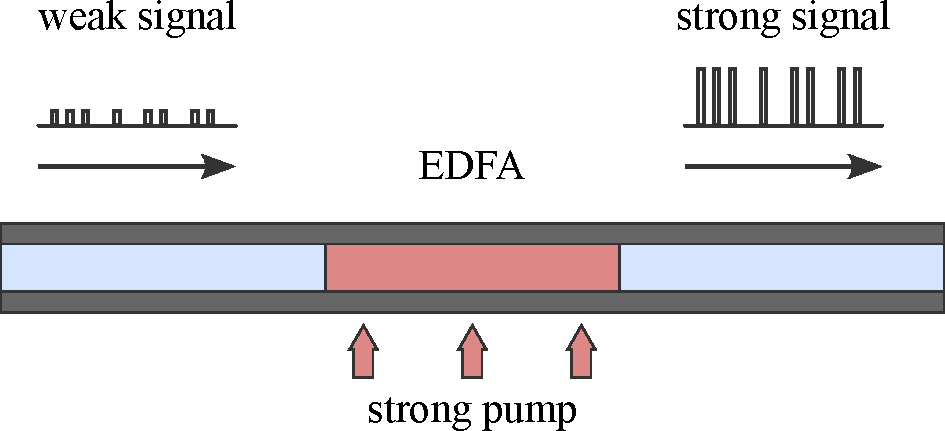
\includegraphics[width=0.6\textwidth]{lesson11/11-4_edfa.pdf}
    \caption[EDFA]{Basic working principle of an erbium-doped fiber amplifier.}
    \label{fig:11-4_edfa}
\end{figure}

\michal{Added gain and active region}
Figure~\ref{fig:11-4_edfa} shows the basics of an EDFA.
Portion of the fiber contains erbium atoms, shown in red. The erbium atoms are pumped strongly to create population inversion, and as the weak signal comes in, it stimulates emission from the red part where we introduced the erbium atoms. In that process, the signal is boosted, and we allow it to travel for another fifty kilometers or so before it needs boosting again.
Commercially available amplifiers are capable of producing gains of up to 40 dB, and are fairly compact with the active region (red in Fig.~\ref{fig:11-4_edfa}) being only few centimeters long.

\michal{Rewrote this paragraph.}
There is one problem with this approach that we have to keep in mind.
EDFAs not only amplify the signal, they also amplify the noise as well.
The excited erbium atoms amplify the signal when they undergo stimulated emission caused by the photons in the signal.
On occasion, these excited atoms emit photons via spontaneous emission as we discussed in Section~\ref{sec:5-2_coherent_vs_incoherent}.
Photons emitted this way travel in a random direction.
When they get emitted in the opposite direction from the incoming signal, it is not a big issue. This does attenuate the signal but at least the spontaneously emitted photons do not pollute the signal.
On the other hand, when the spontaneously emitted photons travel in the same direction as the signal, they contribute to the noise and are responsible for deterioration in the signal-to-noise ratio.
Furthermore, these noisy photons may interact with other excited erbium atoms, stimulating their emission and inadvertently producing more noisy photons.

This is the basic principle of a classical repeater amplifying the signal optically. We will see in the next Section how the sources of noise affect the propagation of signals over long distances in the quantum case.
We will see that the set of challenges that are facing us there are quite different.



\section{Quantum challenges}

In quantum communication, the signal is at the level of individual photons, which is very different from classical communication, where we are sending many, many photons. Photon loss in the fiber therefore becomes a major problem. Classically, if we are communicating and we lose a single photon, it is very insignificant. The whole signal propagates and we can still read it out at the output. However, when this happens in a quantum communication protocol and we lose a single photon, then the entire protocol fails. Go back to, for example E91 or BB84, where the loss of a single photon becomes a huge problem.

So, how can we combat photon loss? We saw that it's possible classically. Let's think whether this is also possible in the quantum communication.

Amplification of a signal worked in classical communication. Can we do that for quantum signals as well? Namely, can we create backup copies of the single photons such that if one gets lost, we can still use the backups in order to proceed with the protocol? We can, but only if we limit ourselves to orthogonal states. If the states that we are sending are, for example, just qubits \ket{} and \ket{1} in some pattern, fine, we can do that and we can create backup copies. But, in quantum communication all the magic happens with non-orthogonal states, and often these states are entangled with some other qubits somewhere else. Therefore, we have to be able to copy arbitrary states, and this is where we hit the roadblock that we saw in Sec.~\ref{sec:8-3_no-cloning}: the no cloning theorem\index{no-cloning theorem}.

Okay, so amplification will not work in quantum communication. How about just sending the photon and hoping for the best?

Let's do a very quick calculation that will demonstrate that this isn't a very good strategy. The probability that we transmit the photon through a fiber over distance $L$, where the attenuation parameter in the fiber is $\alpha$, is given by the expression
\begin{equation}
P_{\text {success }}=10^{-\alpha L / 10}.
\end{equation}

Let's plug in some numbers to give us some intuition of what this probability is. Consider a long fiber of thousand kilometers (which in the context of global communication is not actually that long), and we will assume a best-case scenario where the fiber has ultra-low attenuation of a mere $0.1$ decibels per kilometer. The probability that we actually successfully transmit a single photon is $10^{-10}$. This looks like a very small number, and indeed it is, but to give you some intuition of really how small this number is, let's consider the case of a source that produces one photon every second. Every second we are sending a single photon down the fiber. How long do we need to wait in order for somebody that's at the end of this fiber a thousand kilometers away to actually successfully receive a single photon? Well, we have to wait on average 317 years. You can see that even with ultra-low loss fibers over moderate distances, sending a single photon down the fiber and hoping for the best is not a very good idea.

Loss is only one source of error that we have to contend with in long distance quantum communication. Other sources include unitary errors such as Pauli errors, namely $X$ errors that randomly flip the state of our photons, or $Z$ errors where we introduce some phase to the photons. There is a whole bunch of non-unitary errors, such as coherence, dephasing, relaxation.  Most of these errors we don't have to deal with in classical communication.

So the situation looks quite dire. Is there any hope for long-distance quantum computation? Not quite. We will see in the chapter that quantum problems just require quantum solutions.



\newpage
\begin{exercises}

\exer{Confirm the calculation of 317 years.}

\exer{We suggested that amplifiers are used every 50km or so.  See if you can find more detailed information about the fiber loss and the spacing of amplifiers in real-world deployments and the amount of gain an EDFA can generate.}

\exer{Write some code to simulate mode dispersion of a square wave as it passes down a multimode fiber of length $L$. Be sure to describe your setup and describe any approximations or assumptions you make.  You will want to make as many of the parameters as possible settable by the user.}

\exer{How many photons per second are in one milliwatt of laser power at a wavelength of 1550nm? \rdv{maybe a different chapter.}}

\end{exercises}

